% This document provides the style to be used for a MSc Thesis at the
% Parallel and Distributed Systems group
\documentclass[11pt,twoside,a4paper,openright]{report}

% math packages
\usepackage{amsmath}
\usepackage{amssymb}

% textblocks for title page
\usepackage[absolute]{textpos}

% use babel for proper hyphenation
\usepackage[british]{babel}

% Graphics: different for pdflatex or dvi output, choose one
%%\usepackage[dvips]{graphicx}
%%\usepackage[pdftex]{graphicx}
\usepackage{graphicx}

\usepackage{epstopdf}
\usepackage{rotating}
\usepackage{subfigure}

% FONT
\usepackage[scaled=.92]{helvet}
%\usepackage{times}

% for url's use "\url{http://www.google.com/}"
\usepackage{url}
\usepackage[plainpages=false]{hyperref}



\usepackage{enumitem}





% Information that will be filled in at various points in the report
\newcommand{\reportTitle}{Leveraging VLC for energy disaggregation in Smart Buildings}
\newcommand{\reportAuthor}{Johnny Verhoeff}
\newcommand{\reportEmail}{j.s.c.j.verhoeff@student.tudelft.nl}
\newcommand{\reportUrlEmail}{\href{mailto:\reportEmail}{\reportEmail}}
\newcommand{\reportMSC}{Embedded Systems} %{Embedded Systems}{Computer Engineering}{Computer Science}{Electrical Engineering}
\newcommand{\reportDate}{\today} %TODO: Dit is de datum van uitgifte van final versie aan de afstudeer commissie
\newcommand{\presentationDate}{\today} %TODO: Dit is de datum van de afstudeerpresentatie
\newcommand{\graduationCommittee}{
TODO GRADUATION COMMITTEE & Delft University of Technology \\
TODO GRADUATION COMMITTEE & Delft University of Technology \\
} % The order of listing the names: Graduation prof, supervisor(s), others ordered by title + alphabetical
%examples:
%prof. dr. ir. H. J. Sips (chair) & Delft University of Technology \\
%ir. dr. D. H. J. Epema           & Delft University of Technology \\
\newcommand{\reportAbstract}{TODO ABSTRACT}
\newcommand{\reportKeywords}{VLC, CDMA}

% For pdflatex
\pdfinfo{
   /Author (\reportAuthor)
   /Title  (\reportTitle)
   /Keywords (\reportKeywords)
}

\begin{document}

\pagenumbering{alph}
\pagestyle{empty}


% FRONTCOVER
%%\usepackage[total={210mm,297mm},left=0pt,bottom=0pt,top=0cm,right=0pt,headsep=0pt,head=0pt,showframe]{geometry}

%%\input{preambleL31958}
%%\begin{titlepage}
\begin {textblock*}{210mm}(0mm,0mm)
\noindent

\includegraphics[height=3.2cm]{pics/block}
\sffamily
\vspace{.8cm}
\begin{center}
\Large
Delft University of Technology\\
Master's Thesis in \reportMSC\\
\vspace{2cm}
\parbox{170mm}{\bfseries\centering\Huge\reportTitle}\\
\vspace{1cm}
\parbox{170mm}{\bfseries\centering\reportAuthor}

\end{center}
\end{textblock*}

\begin {textblock*}{210mm}[0.0,1.0](0mm,297mm)
\noindent
\hspace{1.89cm}


\hfill\parbox{5cm}{

\includegraphics[width=5cm]{pics/es_logo_cyan_black_rgb}}
\hspace*{2cm}\\

\vspace*{1.5cm}
\noindent

\includegraphics[width=\textwidth]{pics/TU_border_A4_L_front}
\end{textblock*}

\null\newpage


%%%%%%%%%%%%%%%%%%%%%%%%%%%%%%%%%%%%%%%%%%%%%%%%%%%%%%%%%%%%%%%%%%%%%%%%%%%%%%%
\hoffset=1.63cm
\oddsidemargin=0in
\evensidemargin=0in
\textwidth=5in

%%%%%%%%%%%%%%%%%%%%%%%%%%%%%%%%%%%%%%%%%%%%%%%%%%%%%%%%%%%%%%%%%%%%%%%%%%%%%%%
\parindent=1em

% EMPTY PAGE
\cleardoublepage

\pagestyle{plain}
\pagenumbering{roman}
\setcounter{page}{1}

% TITLE PAGE: page i (hidden)
\begin{titlepage}

  \begin{center}
  \null\vfill
    \begin{center}
    \LARGE{\reportTitle}
    \end{center}

    \vspace{3cm}

    \begin{large}
    Master's Thesis in \reportMSC
    \end{large}

    \vspace{1.5cm}

    \begin{normalsize}
    Embedded Software Section\\
    Faculty of Electrical Engineering, Mathematics and Computer Science\\
    Delft University of Technology\\
    Mekelweg 4, 2628 CD Delft, The Netherlands
    \end{normalsize}

    \vspace{2.0cm}

    \begin{normalsize}
    \reportAuthor \\
    \reportUrlEmail
    \end{normalsize}

    \vspace{1.0cm}

    % <MM> DD, YYYY
    \reportDate             %TODO: Dit is de datum van uitgifte van final versie aan de afstudeer commissie

  \vfill
  \end{center}

\end{titlepage}


% GRADUATION DATA AND ABSTRACT: pages ii and iii (hidden)
%De aankondiging bevat de spreker, titel, plaats, datum en tijd, samenstelling van de afstudeercommissie en een korte samenvatting (maximaal 25 regels).
\thispagestyle{empty}

\noindent \textbf{Author}\\
\begin{tabular}{l}
\reportAuthor{} (\reportUrlEmail)\\
\end{tabular}\\
\noindent \textbf{Title}\\
\begin{tabular}{l}
\reportTitle\\
\end{tabular}\\
\noindent \textbf{MSc presentation}\\
\begin{tabular}{l}
% <MM> DD, YYYY (like \today)
\presentationDate\\
\end{tabular}

\vspace{1.1cm}

\noindent \textbf{Graduation Committee}\\
\begin{tabular}{ll}
\graduationCommittee
\end{tabular}


\begin{abstract} %de abstract bevat alleen een korte samenvatting van de inhoud van het onderzoek
\setcounter{page}{3}
\reportAbstract{}
\end{abstract}

\clearpage

%\setcounter{page}{4}

% EMPTY PAGE: page iv
\cleardoublepage

% OPTIONAL QUOTATION: page v
%\pagestyle{empty}

\null\vfill

\begin{center}
\emph{``TODO QUOTE''} -- TODO QUOTED PERSON
\end{center}

\vspace{10cm}

\clearpage


% EMPTY PAGE: page vi
%\cleardoublepage

% PREFACE: page v
% !TeX root = ../thesis.tex

\chapter*{Preface}
\addcontentsline{toc}{chapter}{Preface}



This Master thesis is the final part of the Master of Science in Embedded Systems program I followed at Delft University of Technology.
Prior to this thesis, I had little knowledge of VLC or energy disaggregation.
Using VLC in combination with energy disaggregation has not been explored yet.
The first steps towards disaggregating individual lights are taken in this thesis.
There are experimental results achieved as well as theoretical results, through simulation.







\vspace{1\baselineskip}

\noindent



First, I would like to thank my loving family, who have support me throughout this nine-month thesis project.
I would also like to thank my advisor Marco Z\'u\~niga Zamalloa and Akshay Narashiman for their guidance to help me finish my thesis.
Finally I want to acknowledge Koen Langendoen and Laura Ramirez Elizondo for being members of my graduation committee.







\vspace{1\baselineskip}

\noindent
Johnny Verhoeff

\vspace{1\baselineskip}

\noindent
Delft, The Netherlands

\noindent
\today

% EMPTY PAGE: page
\cleardoublepage

% TABLE OF CONTENTS: starting at page vii
\tableofcontents

\cleardoublepage

\pagenumbering{arabic}
\setcounter{page}{1}




% INTRODUCTION: page 1
\chapter{Introduction}
\label{chp:introduction}
TODO INTRODUCTION

\vspace{1\baselineskip}

\noindent
TODO ORGANISATIONAL DESCRIPTION OF THESIS



% CHAPTERS ... For instance: History/Prior Work, Design/Implementation, Experiments
\chapter{CHAPTER TITLE}
\label{chp:CHAPTERTITLE}
INTRODUCTION TEXT TO THIS CHAPTER IN WHICH ALL SECTIONS ARE DESCRIBED ROUGHLY (1 SENTENCE EACH).

This chapter describes the ... In Section~\ref{sec:SECTIONTITLE}, examples are given of how to use tables and figures in MSc theses.

\section{SECTION TITLE}
\label{sec:SECTIONTITLE}

Every caption of a table (or figure) should start with a capital letter, and should end with a period. References to tables are given with a capital letter for table, as in ``(see Table~\ref{tab:EXAMPLETABLE})'' or ``in Table~\ref{tab:EXAMPLETABLE}, ...''.

\begin{table}[htb]
\centering
\begin{tabular}{|l|c|r|}
\hline % horizontal line
left aligned & centred & right aligned \\
\hline \hline
12           & 34      & 56            \\
\hline
\end{tabular}
\caption{Complete sentence describing the tabular data.}
\label{tab:EXAMPLETABLE}
\end{table}

References to figures are given with a capital letter for figure, as in ``(see Figure~\ref{fig:EXAMPLEFIGURE})'' or ``in Figure~\ref{fig:EXAMPLEFIGURE}, ...''.

\cite{b}
\cite{a}

\begin{figure}[htb]
% most GNUplot figures need to be rotated, width should be the same throughout the complete document, and no extension is needed

\includegraphics[angle=180,width=\textwidth]{pics/TUD_logo_zw}
\caption{Complete sentence describing the figure thoroughly.}
\label{fig:EXAMPLEFIGURE}
\end{figure}



%!TEX root = ../../thesis.tex

\section{CDMA}
\label{sec:CDMA}

	This section will explain what CDMA is, alternatives and why it is needed.

	When transmitting data from a transmitter to a receiver over a channel, the entire channel is being used for this purpose.
	If one wants to have multiple transmitters transmitting over one channel, there is a problem. 
	The transmitters interfere with each other, this is called multiple access interference (MAI). 
	There are several ways to get around this problem: 

	\begin{itemize}
		\item TDM: Time Division Multiplexing. \\
				Each transmitter gets assigned a time slot, in which it and only it is allowed to transmit, hereby going around the MAI problem.
		\item FDM: Frequency Division Multiplexing. \\
				Each transmitters gets assigned a frequency band. Each transmitter is allowed to transmit the whole time, but only at the assigned frequencies.
		\item CDM: Code Division Multiplexing. \\
				Each transmitter gets assigned a code word. 
				The data first needs to be encoded using the code word and then the transmitter can send his message. 
				Each transmitter can transmit all the time using the entire frequency band. 
				These codes will determine how many transmitters can actually transmit with correct decoding results at the receiver end.
	\end{itemize}

	The distributed network of the VLC LEDs is inherently uncoordinated, since all the LEDs are basically only lights. 
	They have no receiver of any kind. 
	They can only implicitly transmit data by turning the load or the LED on or off.
	Because the LEDs cannot receive data, they cannot be assigned a time slot and therefor we cannot use a TDM scheme.

	An FDM scheme is also not applicable.
	This is because the LEDs do not have an explicit hardware transmitter that can modulate a signal.
	Instead the transmitting is implicitly done via turning the LED on and off.
	So only binary values of the current draw are sent as signals.

	This is where the CDM approach comes into play.
	This scheme allows the multiple LEDs to transmit at the same time.
	But the type of code used here is of importance.
	The code type determines the MAI and what the receiver is able to decode.

	\subsection{Performance metrics of a code}
	\label{subsec:performance-metrics}

		To determine which code is the best for this problem some measures are needed to be able to compare the codes.

		One such a measure is called the correlation.
		Correlation is a measure for determining how much sequence $X$ is similar to sequence $Y$ and can be found in \autoref{eq:correlation}.
		With $L$ being the length of the code and $\tau$ the time-shift.
		When sequence $X$ and $Y$ are the same sequence, we speak of the autocorrelation.
		When they are two different sequences, we speak of the cross-correlation. 

		\begin{equation}
			R(\tau)_{xy} = \displaystyle\sum_{i = 0} ^ {L - 1} x(i) \times y(i + \tau) {\text{  with $\tau = 0, 1, 2, \dotsc, L$}}
			\label{eq:correlation}
		\end{equation}

		The properties of an ideal code set should be, that the autocorrelation for each code in the set should be $0$ for each time-shift $\tau \neq 0$, at $\tau = 0$ the autocorrelation should be $L$.
		The ideal cross-correlation properties should $0$ for every time-shift $\tau$, so that no code interferes with any other code, hereby causing no MAI.

		Other metrics to be considered are the length of the code and how many codes there are in that code set.
		The code length is of importance because each bit a user will transmit must be encoded. 
		So the the message that will be transmitted via the channel will be the length of the code times the length of the data.
		If there are only a few codes in a code set then only a few number of users can transmit which does not scale well. 

	\subsection{Walsh-Hadamard Sequences}

		Walsh-Hadamard sequences are sequences which are created using a Hadamard matrix.
		Hadamard matrices are $n \times n$ matrices which are recursively generated.
		Starting with a $1 \times 1$ matrix: 
		$H_{1} = \begin{bmatrix} 1 \end{bmatrix}$, then 
		$H_{2} = \begin{bmatrix} 1 & 1 \\ 1 & -1 \end{bmatrix}$.
		Or in general: $H_{2n} = \begin{bmatrix} H_n & H_n \\ H_n & -H_n \end{bmatrix}$ \cite{714616}.
		The matrix can also be filled with binary values: zero and one. In that case the general matrix will be: 
		$H_{2n} = \begin{bmatrix} H_n & H_n \\ H_n & \overline{H_n} \end{bmatrix}$

		The Hadamard matrix has the property that every row in the matrix is orthogonal to every other row.
		Hadamard matrices exist for every power of $2$, so the code length is also a power of $2$.
		So for $\tau = 0$, the cross-correlation is $0$, but when $\tau \neq 0$ not all the rows are orthogonal anymore.
		\cite{1182447} proved that an Hadamard matrix of size $2^P$ could be divided into $P + 1$ subsets of rows, where one code could be selected giving $P + 1$ orthogonal codes for each time-shift $\tau$.
		These codes are called Cyclically Orthogonal Walsh Hadamard Codes (COWHC).

		All rows of the matrix have the property that the autocorrelation at $\tau = 0$ is equal to $L$.
		But when $\tau \neq 0$, undesirable behavior occurs as can be seen in \autoref{fig:autocorr-hadamard}.
		The autocorrelation function has several high peaks where only one is desired.
		This means that if a transmitter sends an encoded message with this code and the receiver does not know when in time the start of the message is, the receiver would get false positives for data.

		\begin{figure}
			\centering
			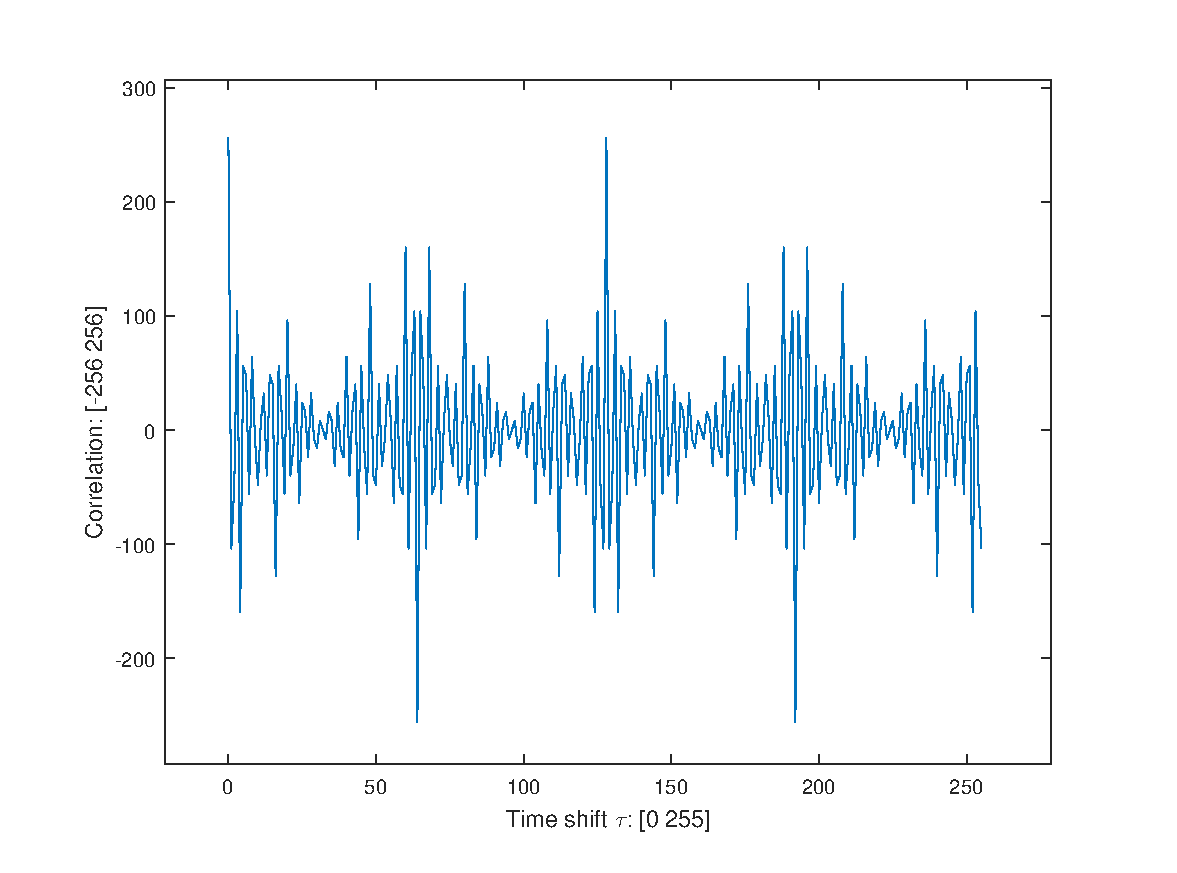
\includegraphics[width=\textwidth]{chapters/CDMA/autocorr-hadamard.eps}
			\caption{Autocorrelation of Hadamard code with index 120 of length 256.}
			\label{fig:autocorr-hadamard}
		\end{figure}

		So only a small subset of the codes have $0$ cross-correlation for every time-shift $\tau$ and the autocorrelation is far from what the ideal code set should have.


	\subsection{PN Sequences}

		PN sequences are sequences where the numbers looks like they are randomly generated but they are easily generated in software or hardware.
		The sequences have the following noise-like properties~\cite{mitra2008pseudo}:

		\begin{itemize}
			\item Balanced \\
					Any PN sequence of length $L = 2^n - 1$ contains exactly $2^{n-1}$ ones and $2^{n-1} - 1$ zeros.

			\item Runs \\
					A run is a subset of the sequence where all the consecutive numbers are the same.
					In any PN sequence, $1/2$ of the runs have length 1, $1/4$ have length 2, $1/8$ have length 3 and so on.

			\item Autocorrelation \\
					The autocorrelation function of a PN sequence will take on two values as can be seen in \autoref{eq:autocorr-pn} and \autoref{fig:autocorr-pn}.


		\end{itemize}

		\begin{equation}
			\label{eq:autocorr-pn}
			R(\tau) = 
				\begin{cases}
					L    & \quad \text{if } \tau = 0 \\
					-1   & \quad \text{if } \tau \neq 0 \\
				\end{cases}
		\end{equation}

		\begin{figure}
			\centering
			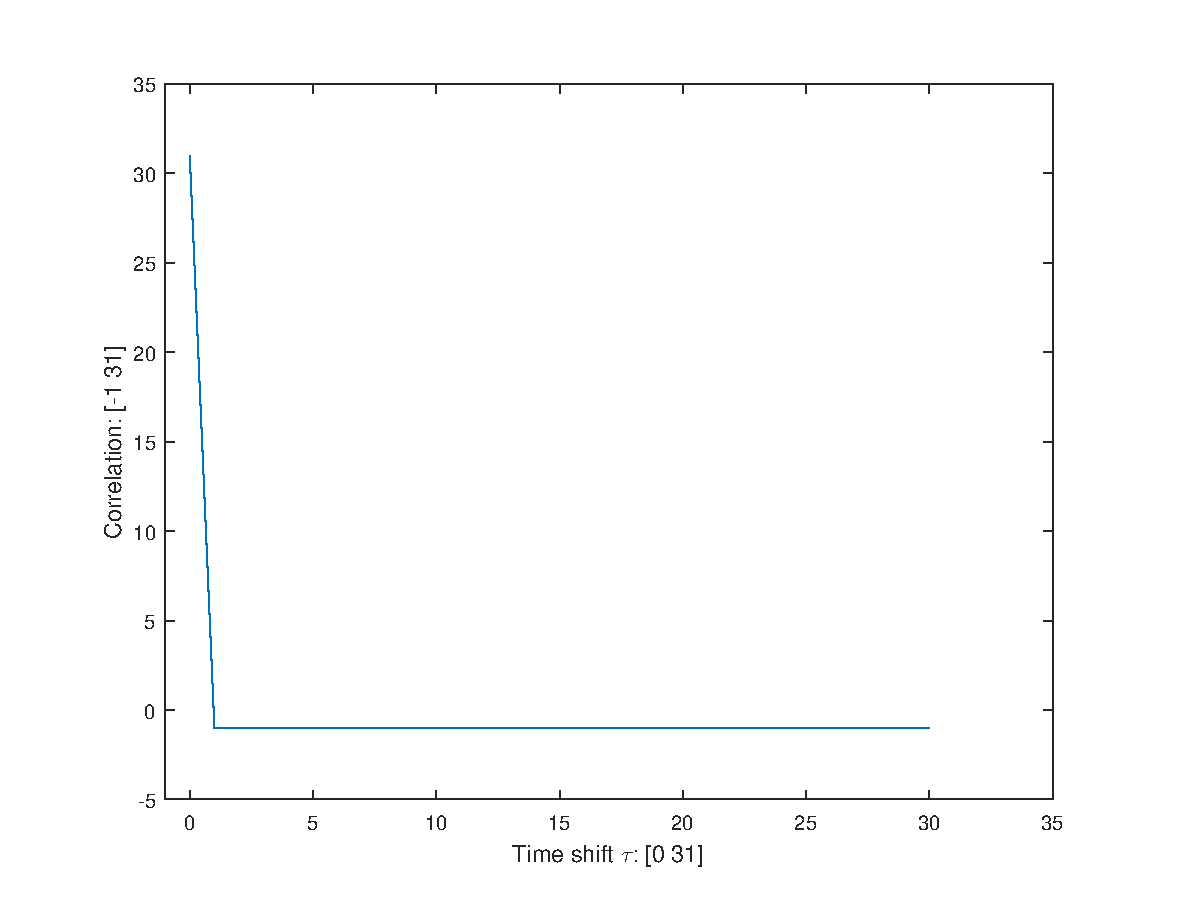
\includegraphics[width=\textwidth]{chapters/CDMA/autocorr-pn.eps}
			\caption{Autocorrelation of PN sequence of length 31.}
			\label{fig:autocorr-pn}
		\end{figure}

		PN sequences are generated using a linear feedback shift register (LFSR) \cite{Wang:1988:LFS:52007.52024}.
		\autoref{fig:lfsr} shows an $n$ length LFSR with some XOR gates attached to it.
		The LFSR is defined entirely by the feedback function, also called a characteristic polynomial.
		It determines the length and the type of sequence generated.
		The polynomial looks like \autoref{eq:lfsr-polynomial}.
		The LFSR in \autoref{fig:lfsr} contains $n$ shift registers and is initiated with a starting seed.
		This seed can be any vector apart from the all zero vector.
		The reason for this is because the XOR function with two zeros as input will output a zero, making the sequence that this LFSR outputs a sequence of all zeros.
		The output of the shift registers are multiplied with the coefficients of the characteristic polynomial ($C_{n-1}, C{n-2}, \dotsc, C_1, C_0$).
		The result output is then fed back into the first shift register, all the bits in the rest of the registers also shift one position and one output bit is created.
		With $n$ number of registers and the zero start vector excluded it takes $2^n - 1$ steps to output the entire sequence before it starts to repeat itself.


		\begin{figure}
			\centering
			\begin{tikzpicture}


				\node[block                  ] (a) {$s_{n-1}$};
				\node[block, right = 1cm of a] (b) {$s_{n-2}$};
				\draw[line] (a.east) -- (b.west) ;

				\node[block, right = 3cm of b] (c) {$s_{1}$};
				\node[block, right = 1cm of c] (d) {$s_{0}$};
				\draw[line] (c.east) -- (d.west) ;

				\draw[dashed, line] (b.east) -- (c.west) ;

				\node[coordinate, right = 2cm of d] (e) {};
				\draw[line] (d.east) -- (e.west) node [midway, above] {output};

				\node[XOR, scale=2, below = 2cm of c] (f) {};
				\draw[line] (c.south) -- (f.north) node [midway, right] {$C_1$};
				\draw[line] (d.south) |- (f.east) node [pos=0.21, right] {$C_0$};

				\node[coordinate, right = 1.5cm of b] (h) {};
				\node[XOR, scale=2, below = 2.5cm of h] (g) {};
				\draw[line] (f.west) -- (g.east) ;
				\draw[dashed, line] (h.south) -- (g.north) ;

				\node[XOR, scale=2, below = 2cm of b] (i) {};
				\node[XOR, scale=2, below = 2cm of a] (k) {};

				\draw[line] (b.south) -- (i.north) node [midway, right] {$C_{n-2}$};
				\draw[line] (g.west) -- (i.east) ;
				
				\draw[line] (i.west) -- (k.east) ;
				\draw[line] (a.south) -- (k.north) node [midway, right] {$C_{n-1}$};

				\node[coordinate, left = 1cm of a] (j) {};
				
				\draw[line] (k.west) -| (j) -- (a.west) ;




			\end{tikzpicture}
			\caption{Linear feedback shifter register of length $n$, with XOR gates.}
			\label{fig:lfsr}
		\end{figure}

		\begin{equation}
			\label{eq:lfsr-polynomial}
			p(x) = x^n + C_{n-1} x^{n-1}  + C_{n-2} x^{n-2} + \dotsc + C_{2} x^{2}  + C_{1} x  + C_{0}
		\end{equation}


		% something about cross correlation....






		






% chapter  (end)

% CONCLUSIONS AND FUTURE WORK
% !TeX root = ../thesis.tex

\chapter{Conclusions and Future Work}
\label{chp:conclusionsandfuturework}

	\section{Conclusions}


	The aim of this thesis is to find out if lights could be identified as being on or off, through the current signature, with the help of VLC and a single smart-meter.
	CDMA codes have been investigated and compared to see which is the best suited for this scenario.
	Two solutions have been discussed to overcome the interference problem that comes with these types of codes.
	When these codes were understood and made usable in software simulations, two practical testbed were developed, for DC and AC, in order to experiment with.
	When the correct codes are used dependent on the size of the system, each individual light in each testbed could be successfully identified as being on or off in a timely manner.
	For larger systems a simulation was performed which shows that there can be made a trade-off between time and accuracy. 
	But the simulation showed that even with a high accuracy, the lights could still be identified in a timely manner.
	%As the testbed only represents a case where only these lights were connected, there is more work to be done when for instance there are also other appliances connected.






\section{Future Work}


This work is only the first step to disaggregate which lights are on and off.
There remains more work to be done, below there are ideas for future work.

	\subsection{Power Limiting Capacitor}

	The solution of using a capacitor in order to limit the power dissipated in the current source, introduced in \autoref{subsubsec:current-source} can be further investigated.
	In particular what the drawbacks or benefits the phase-shifting of current has.
	And if the triggering circuit will still function properly or what the modifications are that need to be made in order for this scheme to work properly.


	\subsection{Other Appliances}

	As the testbeds represents a case where only these lights were connected, the question rises: What will happen when other appliances are connected ?
	These could for example be an incandescent light bulb or a refrigerator.
	To answer that question sample data from \cite{kolter2011redd} could be taken to represent some household appliances and added with the data of the modulation shown from the testbeds.
	Then signal filtering techniques could be performed to try and filter the signal from the modulating lights, given the fact that we know that these lights operate at a certain constant frequency.


	\subsection{Dimming Lights}

	LEDs can be often too bright for a persons liking, so the lights are dimmed.
	Dimming of an LED can be done in two ways: PWM, by lowering the duty cycle and so less power is dissipated by the LED or by limiting the current that flows through the LED.
	Since the LEDs are modulating via an OOK scheme, PWM cannot be used so instead current limiting must be done in order to dim the lights.
	But the CDMA codes are designed to work with each transmitter or LED has the same amplitude or in this case the same current.
	By dimming the LED and changing the current the codes may not work anymore.
	A solution for this can be that each LED will have multiple dimming levels and that for each dimming level other frequencies are used to modulate at.
	A filter can then be used to filter between these LEDs which all have the same amplitude.



	\subsection{Transmitting Data}

	With the current state of this system the LEDs can be identified as being on or off by detecting if their unique code is present or not.
	This can be seen as transmitting data, namely one bit, if the LED is on or off.
	If the LED needs to send other data about the status of the light two approaches can be thought of: 


	\begin{itemize}
		\item The unmodified code assigned to the light will be transmitted for the data-bit `0' and the negation of the code will be transmitted for the data-bit `1'. 
		This gives a problem with the definition of the cross-correlation, which is defined only for the unmodified codes. 
		When the negation of the codes is also used, the cross-correlation between the LEDs that are transmitting is no longer bounded by the mathematical formula and all the calculation on how many LEDs can transmit at the same time can no longer be used with these codes.
		It can be investigated if other codes do have a cross-correlation definition where the negation of the codes is also taken into consideration.

		\item Assign two unique codes from the same set to each light. 
		The lights will send the first code for the data-bit `0' and the second code for the data-bit `1'.
		Since the cross-correlation is defined for the codes from the same set this solution should not yield any problems.
		But further investigation may be required to see if this is a viable solution.
	\end{itemize}


	



















% BIBLIOGRAPHY
%#define SORTED 1
\bibliographystyle{bib/latex8}
\bibliography{bib/mycollection}

%\appendix

%\chapter{TODO APPENDIX NAME}
\label{app:}
Appendix body



\end{document}
